% Created 2026-07-10 Fri 12:55
% Intended LaTeX compiler: pdflatex
\documentclass{article}
\usepackage[utf8]{inputenc}
\usepackage[T1]{fontenc}
\usepackage{graphicx}
\usepackage{longtable}
\usepackage{wrapfig}
\usepackage{rotating}
\usepackage[normalem]{ulem}
\usepackage{amsmath}
\usepackage{amssymb}
\usepackage{capt-of}
\usepackage{hyperref}

\usepackage{fancyhdr}
\usepackage[top=25mm, left=25mm, right=25mm]{geometry}
\usepackage{longtable}
\fancyhead[R]{}
\setlength\headheight{43.0pt}
\usepackage[T1]{fontenc}
\usepackage[utf8]{inputenc}
\usepackage[spanish, ]{babel}
\usepackage[backend=biber]{biblatex}

\author{Echeverría Steven, Jami Mateo, Pérez Martín y Zúñiga Sebastián.}
\date{2026-07-10}
\title{Booteo de Sistema Operativo Linux}
\hypersetup{
 pdfauthor={Echeverría Steven, Jami Mateo, Pérez Martín y Zúñiga Sebastián.},
 pdftitle={Booteo de Sistema Operativo Linux},
 pdfkeywords={},
 pdfsubject={},
 pdfcreator={Emacs 27.1 (Org mode 9.7.5)}, 
 pdflang={Español}}
\begin{document}

\maketitle
\fancyhead[C]{
\includegraphics[scale=0.05]{../imagenes/logoEpn.jpg}\\
ESCUELA POLITÉCNICA NACIONAL\\FACULTAD DE INGENIERÍA DE SISTEMAS\\
ARQUITECTURA DE COMPUTADORES}
\thispagestyle{fancy}




\section{Objetivos}
\label{sec:org9874a85}

\begin{itemize}
\item Aprender a  bootear un sistema operativo Linux

\item Aprender sobre la secuencia de arranque de un computador como la
BIOS y la UEFI
\end{itemize}

\section{Instrucciones}
\label{sec:org18dd05a}
\begin{enumerate}
\item Siga el tutorial para la creación de un booteable de Ubuntu como se
indica en la unidad 9 en el archivo Arranque Ubuntu\footnote{Dependiendo de las características de su computador debe
verificar si al crear el medio booteable para Ubuntu, su sistema
reconoce o acepta para el \emph{Target System}}.

\item Realice un respaldo del código de \emph{BitLocker} utilizando un command
prompt de Windows con permisos de administrador\footnote{Si no respalda el código, no podrá arrancar el disco luego de
reiniciar. Más información en: \href{https://www.partitionwizard.com/disk-recovery/bitlocker-recovery-key-bypass.html }{https://www.partitionwizard.com/disk-recovery/bitlocker-recovery-key-bypass.html}}:

\begin{verbatim}
    manage-bde-protectors C:-get
\end{verbatim}

\item Utilizando su computador o el del laboratorio, siga los pasos
indicados para obtener el booteo desde el USB con el Sistema
Operativo de Ubuntu

\item Realice el boot de Ubuntu desde la memoria USB externa y
seleccione la opción de \emph{Probar Sistema Operativo}.
\item Una vez ingresado active un terminal de Ubuntu: \texttt{Ctrl+ALT+T} y
obtenga las características del computador mediante la ejecución de
los comandos: \texttt{lscpu}, \texttt{lsb\_release -a} y \texttt{lspci}. Obtenga capturas
de la ejecución de los comandos. Luego abra este archivo en WSL y
ejecute los comandos desde los bloques shell. Para insertar un
bloque puede usar la combinación \texttt{C-c C-,}, escoja la opción \texttt{src}
e indique que es del tipo shell.
\end{enumerate}

\section{Desarrollo Emacs}
\label{sec:orge3a5c54}
Se sugiere utilizar la opción \texttt{:fontsize
scriptsize} para dar formato a la ejecución del comando. Por ejemplo,
considere:

\begin{verbatim}
whoami
\end{verbatim}

\begin{verbatim}
sebaszun-epn
\end{verbatim}

\subsection{Comando \texttt{lscpu}}
\label{sec:org86a6fd3}
\begin{verbatim}
 lscpu
\end{verbatim}

\begin{center}
\begin{tabular}{llllllllllllllllllllllllllllllllllllllllllllllllllllllllllllllllllllllllllllllllllllllllllllllllllllllll}
Architecture: & x86\textsubscript{64} &  &  &  &  &  &  &  &  &  &  &  &  &  &  &  &  &  &  &  &  &  &  &  &  &  &  &  &  &  &  &  &  &  &  &  &  &  &  &  &  &  &  &  &  &  &  &  &  &  &  &  &  &  &  &  &  &  &  &  &  &  &  &  &  &  &  &  &  &  &  &  &  &  &  &  &  &  &  &  &  &  &  &  &  &  &  &  &  &  &  &  &  &  &  &  &  &  &  &  &  &  & \\[0pt]
CPU & op-mode(s): & 32-bit, & 64-bit &  &  &  &  &  &  &  &  &  &  &  &  &  &  &  &  &  &  &  &  &  &  &  &  &  &  &  &  &  &  &  &  &  &  &  &  &  &  &  &  &  &  &  &  &  &  &  &  &  &  &  &  &  &  &  &  &  &  &  &  &  &  &  &  &  &  &  &  &  &  &  &  &  &  &  &  &  &  &  &  &  &  &  &  &  &  &  &  &  &  &  &  &  &  &  &  &  &  &  & \\[0pt]
Address & sizes: & 48 & bits & physical, & 48 & bits & virtual &  &  &  &  &  &  &  &  &  &  &  &  &  &  &  &  &  &  &  &  &  &  &  &  &  &  &  &  &  &  &  &  &  &  &  &  &  &  &  &  &  &  &  &  &  &  &  &  &  &  &  &  &  &  &  &  &  &  &  &  &  &  &  &  &  &  &  &  &  &  &  &  &  &  &  &  &  &  &  &  &  &  &  &  &  &  &  &  &  &  &  &  &  &  &  & \\[0pt]
Byte & Order: & Little & Endian &  &  &  &  &  &  &  &  &  &  &  &  &  &  &  &  &  &  &  &  &  &  &  &  &  &  &  &  &  &  &  &  &  &  &  &  &  &  &  &  &  &  &  &  &  &  &  &  &  &  &  &  &  &  &  &  &  &  &  &  &  &  &  &  &  &  &  &  &  &  &  &  &  &  &  &  &  &  &  &  &  &  &  &  &  &  &  &  &  &  &  &  &  &  &  &  &  &  &  & \\[0pt]
CPU(s): & 12 &  &  &  &  &  &  &  &  &  &  &  &  &  &  &  &  &  &  &  &  &  &  &  &  &  &  &  &  &  &  &  &  &  &  &  &  &  &  &  &  &  &  &  &  &  &  &  &  &  &  &  &  &  &  &  &  &  &  &  &  &  &  &  &  &  &  &  &  &  &  &  &  &  &  &  &  &  &  &  &  &  &  &  &  &  &  &  &  &  &  &  &  &  &  &  &  &  &  &  &  &  & \\[0pt]
On-line & CPU(s) & list: & 0-11 &  &  &  &  &  &  &  &  &  &  &  &  &  &  &  &  &  &  &  &  &  &  &  &  &  &  &  &  &  &  &  &  &  &  &  &  &  &  &  &  &  &  &  &  &  &  &  &  &  &  &  &  &  &  &  &  &  &  &  &  &  &  &  &  &  &  &  &  &  &  &  &  &  &  &  &  &  &  &  &  &  &  &  &  &  &  &  &  &  &  &  &  &  &  &  &  &  &  &  & \\[0pt]
Vendor & ID: & AuthenticAMD &  &  &  &  &  &  &  &  &  &  &  &  &  &  &  &  &  &  &  &  &  &  &  &  &  &  &  &  &  &  &  &  &  &  &  &  &  &  &  &  &  &  &  &  &  &  &  &  &  &  &  &  &  &  &  &  &  &  &  &  &  &  &  &  &  &  &  &  &  &  &  &  &  &  &  &  &  &  &  &  &  &  &  &  &  &  &  &  &  &  &  &  &  &  &  &  &  &  &  &  & \\[0pt]
Model & name: & AMD & Ryzen & 5 & 7535HS & with & Radeon & Graphics &  &  &  &  &  &  &  &  &  &  &  &  &  &  &  &  &  &  &  &  &  &  &  &  &  &  &  &  &  &  &  &  &  &  &  &  &  &  &  &  &  &  &  &  &  &  &  &  &  &  &  &  &  &  &  &  &  &  &  &  &  &  &  &  &  &  &  &  &  &  &  &  &  &  &  &  &  &  &  &  &  &  &  &  &  &  &  &  &  &  &  &  &  &  & \\[0pt]
CPU & family: & 25 &  &  &  &  &  &  &  &  &  &  &  &  &  &  &  &  &  &  &  &  &  &  &  &  &  &  &  &  &  &  &  &  &  &  &  &  &  &  &  &  &  &  &  &  &  &  &  &  &  &  &  &  &  &  &  &  &  &  &  &  &  &  &  &  &  &  &  &  &  &  &  &  &  &  &  &  &  &  &  &  &  &  &  &  &  &  &  &  &  &  &  &  &  &  &  &  &  &  &  &  & \\[0pt]
Model: & 68 &  &  &  &  &  &  &  &  &  &  &  &  &  &  &  &  &  &  &  &  &  &  &  &  &  &  &  &  &  &  &  &  &  &  &  &  &  &  &  &  &  &  &  &  &  &  &  &  &  &  &  &  &  &  &  &  &  &  &  &  &  &  &  &  &  &  &  &  &  &  &  &  &  &  &  &  &  &  &  &  &  &  &  &  &  &  &  &  &  &  &  &  &  &  &  &  &  &  &  &  &  & \\[0pt]
Thread(s) & per & core: & 2 &  &  &  &  &  &  &  &  &  &  &  &  &  &  &  &  &  &  &  &  &  &  &  &  &  &  &  &  &  &  &  &  &  &  &  &  &  &  &  &  &  &  &  &  &  &  &  &  &  &  &  &  &  &  &  &  &  &  &  &  &  &  &  &  &  &  &  &  &  &  &  &  &  &  &  &  &  &  &  &  &  &  &  &  &  &  &  &  &  &  &  &  &  &  &  &  &  &  &  & \\[0pt]
Core(s) & per & socket: & 6 &  &  &  &  &  &  &  &  &  &  &  &  &  &  &  &  &  &  &  &  &  &  &  &  &  &  &  &  &  &  &  &  &  &  &  &  &  &  &  &  &  &  &  &  &  &  &  &  &  &  &  &  &  &  &  &  &  &  &  &  &  &  &  &  &  &  &  &  &  &  &  &  &  &  &  &  &  &  &  &  &  &  &  &  &  &  &  &  &  &  &  &  &  &  &  &  &  &  &  & \\[0pt]
Socket(s): & 1 &  &  &  &  &  &  &  &  &  &  &  &  &  &  &  &  &  &  &  &  &  &  &  &  &  &  &  &  &  &  &  &  &  &  &  &  &  &  &  &  &  &  &  &  &  &  &  &  &  &  &  &  &  &  &  &  &  &  &  &  &  &  &  &  &  &  &  &  &  &  &  &  &  &  &  &  &  &  &  &  &  &  &  &  &  &  &  &  &  &  &  &  &  &  &  &  &  &  &  &  &  & \\[0pt]
Stepping: & 1 &  &  &  &  &  &  &  &  &  &  &  &  &  &  &  &  &  &  &  &  &  &  &  &  &  &  &  &  &  &  &  &  &  &  &  &  &  &  &  &  &  &  &  &  &  &  &  &  &  &  &  &  &  &  &  &  &  &  &  &  &  &  &  &  &  &  &  &  &  &  &  &  &  &  &  &  &  &  &  &  &  &  &  &  &  &  &  &  &  &  &  &  &  &  &  &  &  &  &  &  &  & \\[0pt]
BogoMIPS: & 6587.45 &  &  &  &  &  &  &  &  &  &  &  &  &  &  &  &  &  &  &  &  &  &  &  &  &  &  &  &  &  &  &  &  &  &  &  &  &  &  &  &  &  &  &  &  &  &  &  &  &  &  &  &  &  &  &  &  &  &  &  &  &  &  &  &  &  &  &  &  &  &  &  &  &  &  &  &  &  &  &  &  &  &  &  &  &  &  &  &  &  &  &  &  &  &  &  &  &  &  &  &  &  & \\[0pt]
Flags: & fpu & vme & de & pse & tsc & msr & pae & mce & cx8 & apic & sep & mtrr & pge & mca & cmov & pat & pse36 & clflush & mmx & fxsr & sse & sse2 & ht & syscall & nx & mmxext & fxsr\textsubscript{opt} & pdpe1gb & rdtscp & lm & constant\textsubscript{tsc} & rep\textsubscript{good} & nopl & tsc\textsubscript{reliable} & nonstop\textsubscript{tsc} & cpuid & extd\textsubscript{apicid} & tsc\textsubscript{known}\textsubscript{freq} & pni & pclmulqdq & ssse3 & fma & cx16 & sse4\textsubscript{1} & sse4\textsubscript{2} & movbe & popcnt & aes & xsave & avx & f16c & rdrand & hypervisor & lahf\textsubscript{lm} & cmp\textsubscript{legacy} & svm & cr8\textsubscript{legacy} & abm & sse4a & misalignsse & 3dnowprefetch & osvw & topoext & perfctr\textsubscript{core} & ssbd & ibrs & ibpb & stibp & vmmcall & fsgsbase & bmi1 & avx2 & smep & bmi2 & erms & invpcid & rdseed & adx & smap & clflushopt & clwb & sha\textsubscript{ni} & xsaveopt & xsavec & xgetbv1 & xsaves & clzero & xsaveerptr & arat & npt & nrip\textsubscript{save} & tsc\textsubscript{scale} & vmcb\textsubscript{clean} & flushbyasid & decodeassists & pausefilter & pfthreshold & v\textsubscript{vmsave}\textsubscript{vmload} & umip & vaes & vpclmulqdq & rdpid & fsrm\\[0pt]
Virtualization: & AMD-V &  &  &  &  &  &  &  &  &  &  &  &  &  &  &  &  &  &  &  &  &  &  &  &  &  &  &  &  &  &  &  &  &  &  &  &  &  &  &  &  &  &  &  &  &  &  &  &  &  &  &  &  &  &  &  &  &  &  &  &  &  &  &  &  &  &  &  &  &  &  &  &  &  &  &  &  &  &  &  &  &  &  &  &  &  &  &  &  &  &  &  &  &  &  &  &  &  &  &  &  &  & \\[0pt]
Hypervisor & vendor: & Microsoft &  &  &  &  &  &  &  &  &  &  &  &  &  &  &  &  &  &  &  &  &  &  &  &  &  &  &  &  &  &  &  &  &  &  &  &  &  &  &  &  &  &  &  &  &  &  &  &  &  &  &  &  &  &  &  &  &  &  &  &  &  &  &  &  &  &  &  &  &  &  &  &  &  &  &  &  &  &  &  &  &  &  &  &  &  &  &  &  &  &  &  &  &  &  &  &  &  &  &  &  & \\[0pt]
Virtualization & type: & full &  &  &  &  &  &  &  &  &  &  &  &  &  &  &  &  &  &  &  &  &  &  &  &  &  &  &  &  &  &  &  &  &  &  &  &  &  &  &  &  &  &  &  &  &  &  &  &  &  &  &  &  &  &  &  &  &  &  &  &  &  &  &  &  &  &  &  &  &  &  &  &  &  &  &  &  &  &  &  &  &  &  &  &  &  &  &  &  &  &  &  &  &  &  &  &  &  &  &  &  & \\[0pt]
L1d & cache: & 192 & KiB & (6 & instances) &  &  &  &  &  &  &  &  &  &  &  &  &  &  &  &  &  &  &  &  &  &  &  &  &  &  &  &  &  &  &  &  &  &  &  &  &  &  &  &  &  &  &  &  &  &  &  &  &  &  &  &  &  &  &  &  &  &  &  &  &  &  &  &  &  &  &  &  &  &  &  &  &  &  &  &  &  &  &  &  &  &  &  &  &  &  &  &  &  &  &  &  &  &  &  &  &  & \\[0pt]
L1i & cache: & 192 & KiB & (6 & instances) &  &  &  &  &  &  &  &  &  &  &  &  &  &  &  &  &  &  &  &  &  &  &  &  &  &  &  &  &  &  &  &  &  &  &  &  &  &  &  &  &  &  &  &  &  &  &  &  &  &  &  &  &  &  &  &  &  &  &  &  &  &  &  &  &  &  &  &  &  &  &  &  &  &  &  &  &  &  &  &  &  &  &  &  &  &  &  &  &  &  &  &  &  &  &  &  &  & \\[0pt]
L2 & cache: & 3 & MiB & (6 & instances) &  &  &  &  &  &  &  &  &  &  &  &  &  &  &  &  &  &  &  &  &  &  &  &  &  &  &  &  &  &  &  &  &  &  &  &  &  &  &  &  &  &  &  &  &  &  &  &  &  &  &  &  &  &  &  &  &  &  &  &  &  &  &  &  &  &  &  &  &  &  &  &  &  &  &  &  &  &  &  &  &  &  &  &  &  &  &  &  &  &  &  &  &  &  &  &  &  & \\[0pt]
L3 & cache: & 16 & MiB & (1 & instance) &  &  &  &  &  &  &  &  &  &  &  &  &  &  &  &  &  &  &  &  &  &  &  &  &  &  &  &  &  &  &  &  &  &  &  &  &  &  &  &  &  &  &  &  &  &  &  &  &  &  &  &  &  &  &  &  &  &  &  &  &  &  &  &  &  &  &  &  &  &  &  &  &  &  &  &  &  &  &  &  &  &  &  &  &  &  &  &  &  &  &  &  &  &  &  &  &  & \\[0pt]
NUMA & node(s): & 1 &  &  &  &  &  &  &  &  &  &  &  &  &  &  &  &  &  &  &  &  &  &  &  &  &  &  &  &  &  &  &  &  &  &  &  &  &  &  &  &  &  &  &  &  &  &  &  &  &  &  &  &  &  &  &  &  &  &  &  &  &  &  &  &  &  &  &  &  &  &  &  &  &  &  &  &  &  &  &  &  &  &  &  &  &  &  &  &  &  &  &  &  &  &  &  &  &  &  &  &  & \\[0pt]
NUMA & node0 & CPU(s): & 0-11 &  &  &  &  &  &  &  &  &  &  &  &  &  &  &  &  &  &  &  &  &  &  &  &  &  &  &  &  &  &  &  &  &  &  &  &  &  &  &  &  &  &  &  &  &  &  &  &  &  &  &  &  &  &  &  &  &  &  &  &  &  &  &  &  &  &  &  &  &  &  &  &  &  &  &  &  &  &  &  &  &  &  &  &  &  &  &  &  &  &  &  &  &  &  &  &  &  &  &  & \\[0pt]
Vulnerability & Gather & data & sampling: & Not & affected &  &  &  &  &  &  &  &  &  &  &  &  &  &  &  &  &  &  &  &  &  &  &  &  &  &  &  &  &  &  &  &  &  &  &  &  &  &  &  &  &  &  &  &  &  &  &  &  &  &  &  &  &  &  &  &  &  &  &  &  &  &  &  &  &  &  &  &  &  &  &  &  &  &  &  &  &  &  &  &  &  &  &  &  &  &  &  &  &  &  &  &  &  &  &  &  &  & \\[0pt]
Vulnerability & Itlb & multihit: & Not & affected &  &  &  &  &  &  &  &  &  &  &  &  &  &  &  &  &  &  &  &  &  &  &  &  &  &  &  &  &  &  &  &  &  &  &  &  &  &  &  &  &  &  &  &  &  &  &  &  &  &  &  &  &  &  &  &  &  &  &  &  &  &  &  &  &  &  &  &  &  &  &  &  &  &  &  &  &  &  &  &  &  &  &  &  &  &  &  &  &  &  &  &  &  &  &  &  &  &  & \\[0pt]
Vulnerability & L1tf: & Not & affected &  &  &  &  &  &  &  &  &  &  &  &  &  &  &  &  &  &  &  &  &  &  &  &  &  &  &  &  &  &  &  &  &  &  &  &  &  &  &  &  &  &  &  &  &  &  &  &  &  &  &  &  &  &  &  &  &  &  &  &  &  &  &  &  &  &  &  &  &  &  &  &  &  &  &  &  &  &  &  &  &  &  &  &  &  &  &  &  &  &  &  &  &  &  &  &  &  &  &  & \\[0pt]
Vulnerability & Mds: & Not & affected &  &  &  &  &  &  &  &  &  &  &  &  &  &  &  &  &  &  &  &  &  &  &  &  &  &  &  &  &  &  &  &  &  &  &  &  &  &  &  &  &  &  &  &  &  &  &  &  &  &  &  &  &  &  &  &  &  &  &  &  &  &  &  &  &  &  &  &  &  &  &  &  &  &  &  &  &  &  &  &  &  &  &  &  &  &  &  &  &  &  &  &  &  &  &  &  &  &  &  & \\[0pt]
Vulnerability & Meltdown: & Not & affected &  &  &  &  &  &  &  &  &  &  &  &  &  &  &  &  &  &  &  &  &  &  &  &  &  &  &  &  &  &  &  &  &  &  &  &  &  &  &  &  &  &  &  &  &  &  &  &  &  &  &  &  &  &  &  &  &  &  &  &  &  &  &  &  &  &  &  &  &  &  &  &  &  &  &  &  &  &  &  &  &  &  &  &  &  &  &  &  &  &  &  &  &  &  &  &  &  &  &  & \\[0pt]
Vulnerability & Mmio & stale & data: & Not & affected &  &  &  &  &  &  &  &  &  &  &  &  &  &  &  &  &  &  &  &  &  &  &  &  &  &  &  &  &  &  &  &  &  &  &  &  &  &  &  &  &  &  &  &  &  &  &  &  &  &  &  &  &  &  &  &  &  &  &  &  &  &  &  &  &  &  &  &  &  &  &  &  &  &  &  &  &  &  &  &  &  &  &  &  &  &  &  &  &  &  &  &  &  &  &  &  &  & \\[0pt]
Vulnerability & Reg & file & data & sampling: & Not & affected &  &  &  &  &  &  &  &  &  &  &  &  &  &  &  &  &  &  &  &  &  &  &  &  &  &  &  &  &  &  &  &  &  &  &  &  &  &  &  &  &  &  &  &  &  &  &  &  &  &  &  &  &  &  &  &  &  &  &  &  &  &  &  &  &  &  &  &  &  &  &  &  &  &  &  &  &  &  &  &  &  &  &  &  &  &  &  &  &  &  &  &  &  &  &  &  & \\[0pt]
Vulnerability & Retbleed: & Not & affected &  &  &  &  &  &  &  &  &  &  &  &  &  &  &  &  &  &  &  &  &  &  &  &  &  &  &  &  &  &  &  &  &  &  &  &  &  &  &  &  &  &  &  &  &  &  &  &  &  &  &  &  &  &  &  &  &  &  &  &  &  &  &  &  &  &  &  &  &  &  &  &  &  &  &  &  &  &  &  &  &  &  &  &  &  &  &  &  &  &  &  &  &  &  &  &  &  &  &  & \\[0pt]
Vulnerability & Spec & rstack & overflow: & Vulnerable: & Safe & RET, & no & microcode &  &  &  &  &  &  &  &  &  &  &  &  &  &  &  &  &  &  &  &  &  &  &  &  &  &  &  &  &  &  &  &  &  &  &  &  &  &  &  &  &  &  &  &  &  &  &  &  &  &  &  &  &  &  &  &  &  &  &  &  &  &  &  &  &  &  &  &  &  &  &  &  &  &  &  &  &  &  &  &  &  &  &  &  &  &  &  &  &  &  &  &  &  &  & \\[0pt]
Vulnerability & Spec & store & bypass: & Mitigation; & Speculative & Store & Bypass & disabled & via & prctl &  &  &  &  &  &  &  &  &  &  &  &  &  &  &  &  &  &  &  &  &  &  &  &  &  &  &  &  &  &  &  &  &  &  &  &  &  &  &  &  &  &  &  &  &  &  &  &  &  &  &  &  &  &  &  &  &  &  &  &  &  &  &  &  &  &  &  &  &  &  &  &  &  &  &  &  &  &  &  &  &  &  &  &  &  &  &  &  &  &  &  &  & \\[0pt]
Vulnerability & Spectre & v1: & Mitigation; & usercopy/swapgs & barriers & and & \_\textsubscript{user} & pointer & sanitization &  &  &  &  &  &  &  &  &  &  &  &  &  &  &  &  &  &  &  &  &  &  &  &  &  &  &  &  &  &  &  &  &  &  &  &  &  &  &  &  &  &  &  &  &  &  &  &  &  &  &  &  &  &  &  &  &  &  &  &  &  &  &  &  &  &  &  &  &  &  &  &  &  &  &  &  &  &  &  &  &  &  &  &  &  &  &  &  &  &  &  &  &  & \\[0pt]
Vulnerability & Spectre & v2: & Mitigation; & Retpolines; & IBPB & conditional; & IBRS\textsubscript{FW}; & STIBP & always-on; & RSB & filling; & PBRSB-eIBRS & Not & affected; & BHI & Not & affected &  &  &  &  &  &  &  &  &  &  &  &  &  &  &  &  &  &  &  &  &  &  &  &  &  &  &  &  &  &  &  &  &  &  &  &  &  &  &  &  &  &  &  &  &  &  &  &  &  &  &  &  &  &  &  &  &  &  &  &  &  &  &  &  &  &  &  &  &  &  &  &  &  &  &  &  &  &  &  &  &  &  &  &  &  & \\[0pt]
Vulnerability & Srbds: & Not & affected &  &  &  &  &  &  &  &  &  &  &  &  &  &  &  &  &  &  &  &  &  &  &  &  &  &  &  &  &  &  &  &  &  &  &  &  &  &  &  &  &  &  &  &  &  &  &  &  &  &  &  &  &  &  &  &  &  &  &  &  &  &  &  &  &  &  &  &  &  &  &  &  &  &  &  &  &  &  &  &  &  &  &  &  &  &  &  &  &  &  &  &  &  &  &  &  &  &  &  & \\[0pt]
Vulnerability & Tsx & async & abort: & Not & affected &  &  &  &  &  &  &  &  &  &  &  &  &  &  &  &  &  &  &  &  &  &  &  &  &  &  &  &  &  &  &  &  &  &  &  &  &  &  &  &  &  &  &  &  &  &  &  &  &  &  &  &  &  &  &  &  &  &  &  &  &  &  &  &  &  &  &  &  &  &  &  &  &  &  &  &  &  &  &  &  &  &  &  &  &  &  &  &  &  &  &  &  &  &  &  &  &  & \\[0pt]
\end{tabular}
\end{center}

\subsection{Comando \texttt{lsb\_release}}
\label{sec:org8c1c595}
\begin{verbatim}
    lsb_release -a
\end{verbatim}

\begin{center}
\begin{tabular}{ll}
Distributor ID: & Ubuntu\\[0pt]
Description: & Ubuntu 24.04.4 LTS\\[0pt]
Release: & 24.04\\[0pt]
Codename: & noble\\[0pt]
\end{tabular}
\end{center}


\subsection{Comando \texttt{lspci}}
\label{sec:org361823c}
\begin{verbatim}
   lspci
\end{verbatim}

\begin{center}
\begin{tabular}{rrllllllrllr}
0d65:00:00.0 & System & peripheral: & Red & Hat, & Inc. & Virtio & file & system & (rev & 01) & \\[0pt]
5582:00:00.0 & SCSI & storage & controller: & Red & Hat, & Inc. & Virtio & 1.0 & console & (rev & 01)\\[0pt]
5cce:00:00.0 & 3D & controller: & Microsoft & Corporation & Basic & Render & Driver &  &  &  & \\[0pt]
9694:00:00.0 & 3D & controller: & Microsoft & Corporation & Basic & Render & Driver &  &  &  & \\[0pt]
\end{tabular}
\end{center}

\section{Desarrollo Capturas}
\label{sec:org597d1db}
Coloque las capturas de los resultados obtenidos en los
terminales. Para esto recuerde utilizar dobles corchetes y escribir el
\emph{path} hacia la imagen. Pruebe a utilizar YASnipet para generar el
siguiente código para descripción de la figura. Para esto puede
escriba \texttt{fig\_} seguido de la combinación de teclas \texttt{C-TAB}, finalmente
coloque la dirección de la imagen. Las figuras se presentaron en la
siguiente parte de la consulta, por motivos de espacio y orientación
en LaTex.

\section{Consulta}
\label{sec:orgd5cc80a}
Describa que hacen y para qué sirven los comandos utilizados en la práctica

\begin{description}
\item[{lscpu}] Muestra información detallada sobre la arquitectura del
procesador (CPU) del sistema. Recopila datos directamente
de los archivos internos del sistema (/proc/cpuinfo) y de la
arquitectura de la máquina para presentar un resumen estructurado
del hardware de procesamiento. Además, sirve para conocer la
potencia, la estructura y las capacidades técnicas del procesador.
\end{description}
\begin{figure}[htbp]
\centering
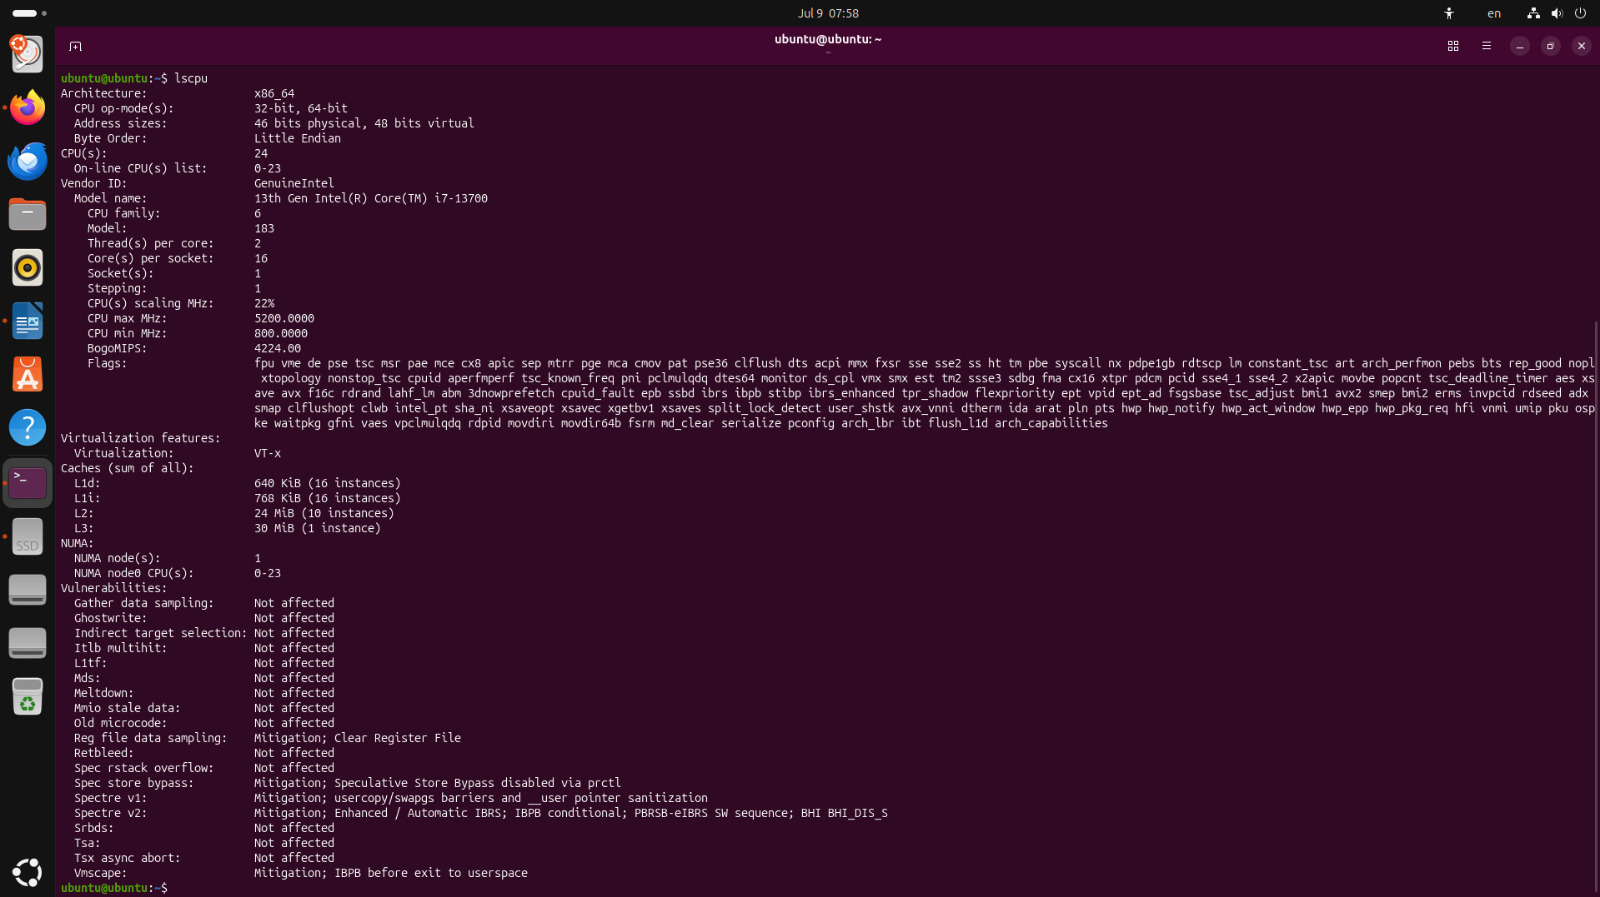
\includegraphics[width=.9\linewidth]{./imagenes/Figura1_UbuntuT.jpeg}
\caption{\label{fig:org393eadb}lscpu}
\end{figure}

\begin{description}
\item[{lspci}] Muestra una lista detallada de todos los dispositivos
conectados a los puertos PCI y PCI Express de la placa base.
De igual forma, ayuda a identificar los componentes físicos de la máquina.

\item[{lsb\textsubscript{release} -a}] Muestra información específica sobre la
distribución de Linux instalada.Permite verificar la versión exacta
del sistema operativo y su nombre en clave.
\end{description}

\begin{figure}[htbp]
\centering
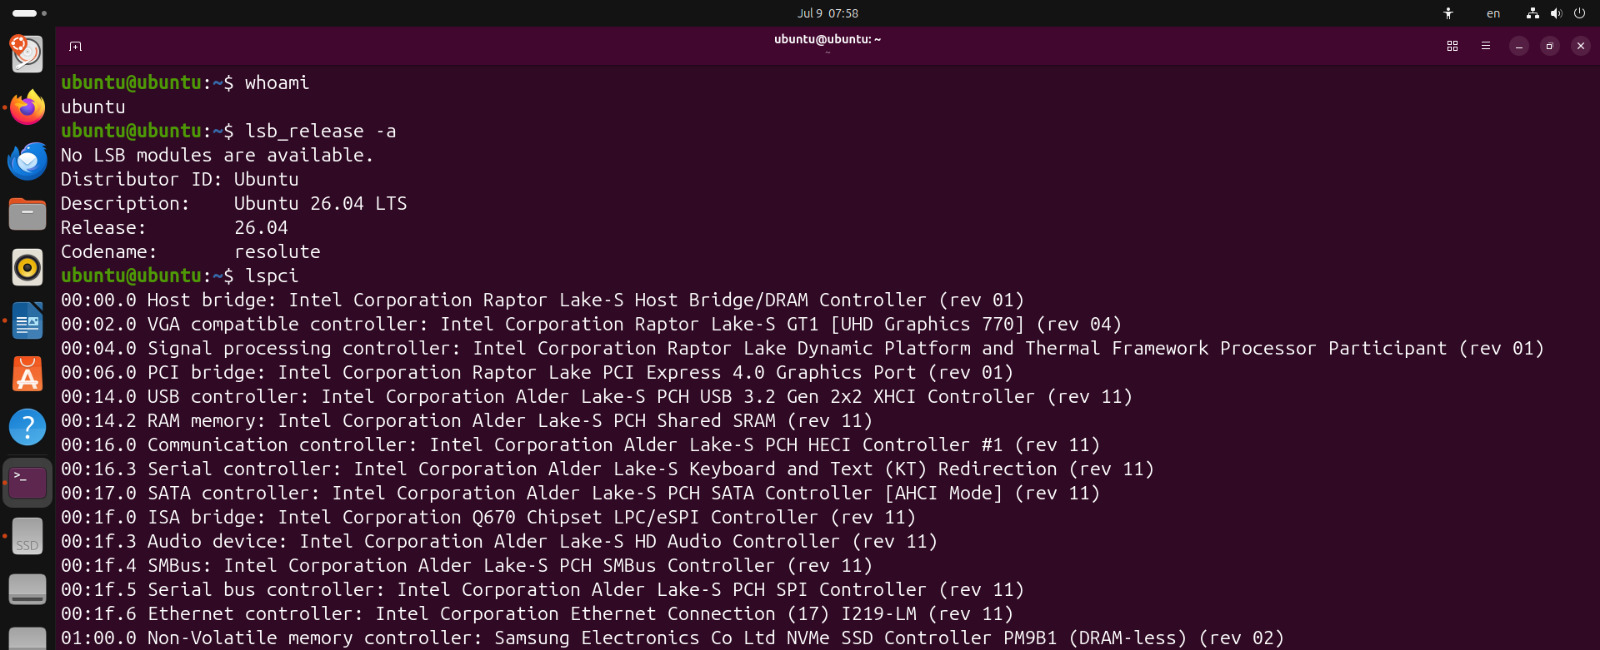
\includegraphics[width=.9\linewidth]{./imagenes/Figura2_UbuntuT.jpeg}
\caption{\label{fig:orgf3b6f78}lsb\textsubscript{release} -a y lspci}
\end{figure}
\end{document}
